\documentclass[10pt]{article}
\usepackage[margin=1in]{geometry}
\usepackage{amsmath,amssymb,bm}
\usepackage{booktabs}
\usepackage{graphicx}
\usepackage{hyperref}
\usepackage{enumitem}
\usepackage{caption}
\usepackage{titlesec}

\hypersetup{colorlinks=true,linkcolor=blue,urlcolor=blue,citecolor=blue}
\setlength{\parskip}{0.30em}
\setlength{\parindent}{0pt}
\captionsetup{font=small,labelfont=bf,skip=4pt}
\titlespacing*{\section}{0pt}{0.65em}{0.22em}
\titlespacing*{\subsection}{0pt}{0.45em}{0.15em}

\begin{document}

\begin{center}
\vspace*{-1.0em}
{\large\textbf{Taming Ill-Conditioning in PINNs: Exact Second-Order Descent via Gauss--Newton}\par}
\end{center}
\vspace{0.1em}

\section{Conclusions of Rathore et al.\ (ICML 2024)}

A Physics-Informed Neural Network (PINN) approximates an unknown PDE solution $u^*(x)$ with a neural network $u_\theta(x)$ ($\theta \in \mathbb{R}^D$) by minimizing the mean-squared PDE residual, boundary, and initial conditions across $N$ collocation points:
\begin{equation}
L(\theta) = \frac{1}{2}\|r(\theta)\|_2^2 = \frac{1}{2}\sum_{i=1}^N r_i(\theta)^2.
\label{eq:loss}
\end{equation}
Unlike supervised learning with noisy labels, forward PINNs are deterministic approximation tasks requiring $L(\theta) \to 0$ for physical fidelity. Rathore et al.\ study why gradient methods struggle to achieve this precision and establish three primary takeaways:
\begin{enumerate}[leftmargin=1.4em,itemsep=0.10em,topsep=0.12em]
    \item \textbf{Differential operators induce severe loss landscape ill-conditioning:} Applying a differential operator $\mathcal{D}[u_\theta]$ (e.g., $\partial_{xx}$, $\partial_{xxxx}$, or $\partial_{tt} - c^2 \partial_{xx}$) amplifies high-frequency modes and stretches the eigenvalue spectrum of the loss Hessian $H_L(\theta) = \nabla^2 L(\theta)$ across $10^3\text{--}10^5+$ orders of magnitude, generating narrow, anisotropic canyons.
    \item \textbf{First-order methods stall inside ill-conditioned canyons:} Near initialization, Adam navigates past non-convex saddle points into a promising basin, but its gradient is dominated by steep canyon walls, oscillating transversely and stalling at $10^{-2}\text{--}10^{-4}$ relative $L^2$ error.
    \item \textbf{Second-order curvature scaling is required to restore isotropic descent:} Rescaling descent steps by inverse curvature compresses the stretched Hessian spectrum by $>10^3\times$. Because quasi-Newton \texttt{L-BFGS} relies on gradient history and stalls along narrow valleys, Rathore et al.\ introduce \textbf{NysNewton-CG (\texttt{NNCG})}---solving $(H_L + \mu I) d = -\nabla L$ via Nystr\"om-preconditioned Conjugate Gradient (CG) following an \texttt{Adam -> L-BFGS} warm-up.
\end{enumerate}

\section{Problems with \texttt{NNCG}}

To understand why \texttt{NNCG} is both computationally demanding and fragile away from the minimizer, we examine the analytic Hessian of the least-squares objective $L(\theta) = \frac{1}{2}\|r(\theta)\|_2^2$:
\begin{equation}
H_L(\theta) = \underbrace{J(\theta)^T J(\theta)}_{\text{Gauss--Newton matrix } (\succeq 0)} + \underbrace{\sum_{i=1}^N r_i(\theta) \, \nabla^2 r_i(\theta)}_{\text{residual curvature (indefinite)}}, \qquad J(\theta) = \frac{\partial r}{\partial \theta} \in \mathbb{R}^{N \times D}.
\label{eq:hessian_split}
\end{equation}
Operating directly on the full loss Hessian $H_L(\theta)$ introduces three structural deficiencies into \texttt{NNCG}:
\begin{enumerate}[leftmargin=1.4em,itemsep=0.10em,topsep=0.10em]
    \item \textbf{Indefiniteness violates descent and derails Conjugate Gradient:} Whenever $r(\theta) \neq 0$ (early in training or under measurement noise), the residual curvature term $\sum_{i=1}^N r_i \nabla^2 r_i(\theta)$ introduces negative eigenvalues into $H_L(\theta)$. Indefiniteness violates the descent condition $d^T \nabla L < 0$, directs Newton steps toward saddle points, and invalidates Conjugate Gradient (which strictly requires positive definiteness), necessitating thousands of first-order preconditioning steps.
    \item \textbf{Dense rank-$D$ residual curvature prevents dual dimension reduction:} Because $\sum_{i=1}^N r_i \nabla^2 r_i(\theta)$ is a dense $D \times D$ operator of full rank, $H_L(\theta)$ cannot be reduced to the collocation dimension $N \times N$. Even when $N \ll D$, materializing $H_L(\theta)$ scales as $\mathcal{O}(D^2)$ memory and $\mathcal{O}(D)$ second-derivative passes, forcing \texttt{NNCG} to employ low-rank Krylov approximations.
    \item \textbf{Second-derivative operator differentiation creates severe overhead:} Because $r(\theta)$ contains spatial derivatives, applying $H_L(\theta)$ in matrix-free CG requires evaluating second-derivative operator passes sequentially, yielding per-step runtimes orders of magnitude slower than first-order updates.
\end{enumerate}

\section{Exact Gauss--Newton (\texttt{EGN}) Algorithm}

In language and vision models, parameter dimension $D$ ($10^8\text{--}10^{11}$) and dataset size $N$ ($10^6\text{--}10^{12}$) necessitate first-order methods. \textbf{Practical PINNs inhabit the opposite regime:} compact networks ($D \sim 5\text{k}\text{--}50\text{k}$) evaluated on moderate collocation sets ($N \sim 500\text{--}10{,}000$, frequently with $N < D$).

Crucially, in forward PINNs, driving the residual toward zero ($r(\theta^*) \to 0$) implies that \textbf{the loss Hessian asymptotically converges to the Gauss--Newton matrix:}
\begin{equation}
H_L(\theta) = J(\theta)^T J(\theta) + \sum_{i=1}^N r_i(\theta) \, \nabla^2 r_i(\theta) \;\xrightarrow{\|r(\theta)\|_2 \to 0}\; J(\theta)^T J(\theta).
\label{eq:asymptotic}
\end{equation}
By discarding the residual curvature $\sum_i r_i \nabla^2 r_i(\theta)$, the linear system $(J^T J + \mu I_D) d = -J^T r$ can be solved \textbf{identically in whichever dimension $\min(N, D)$ is smaller} via the push-through identity:
\begin{equation}
d = \underbrace{-(J^T J + \mu I_D)^{-1} J^T r}_{\text{Primal solve } (D \times D\text{, when } D \le N)} \;=\; \underbrace{-J^T (J J^T + \mu I_N)^{-1} r}_{\text{Dual solve } (N \times N\text{, when } N < D)}.
\label{eq:primal_dual}
\end{equation}
Discarding the indefinite residual curvature yields three foundational mathematical properties:
\begin{enumerate}[leftmargin=1.4em,itemsep=0.10em,topsep=0.10em]
    \item \textbf{Zero approximation error at a clean PDE solution ($r(\theta^*) = 0$):} The gradient $\nabla L(\theta) = J(\theta)^T r(\theta)$ is exact, and as $r_i \to 0$, $\sum_i r_i \nabla^2 r_i(\theta) \to 0$ automatically, so \textbf{$J^T J$ equals the exact Hessian $H_L$ at the solution}.
    \item \textbf{Immunity to saddle points and noise away from $r = 0$:} When $r_i \neq 0$ (early in training or under additive noise $\epsilon_i$), $\sum_i r_i \nabla^2 r_i$ injects negative eigenvalues into $H_L$ that force \texttt{NNCG} to add heavy damping $\mu$ or abort CG early. Because $J^T J \succeq 0$ does not depend on $r_i$, every \texttt{EGN} step points strictly downhill from random initialization.
    \item \textbf{Exact full-rank Cholesky in $\min(N, D)$ vs.\ low-rank CG approximation:} \texttt{NNCG} only approximates $(H_L + \mu I)^{-1}$ via a rank-60 Nystr\"om preconditioner and iterative CG, whereas \textbf{\texttt{EGN}} directly factors the full $\min(N, D) \times \min(N, D)$ matrix via Cholesky, inverting \emph{all} curvature directions simultaneously using only first derivatives of $r(\theta)$.
\end{enumerate}

\begin{figure}[!htb]
    \centering
    \vspace{-0.2em}
    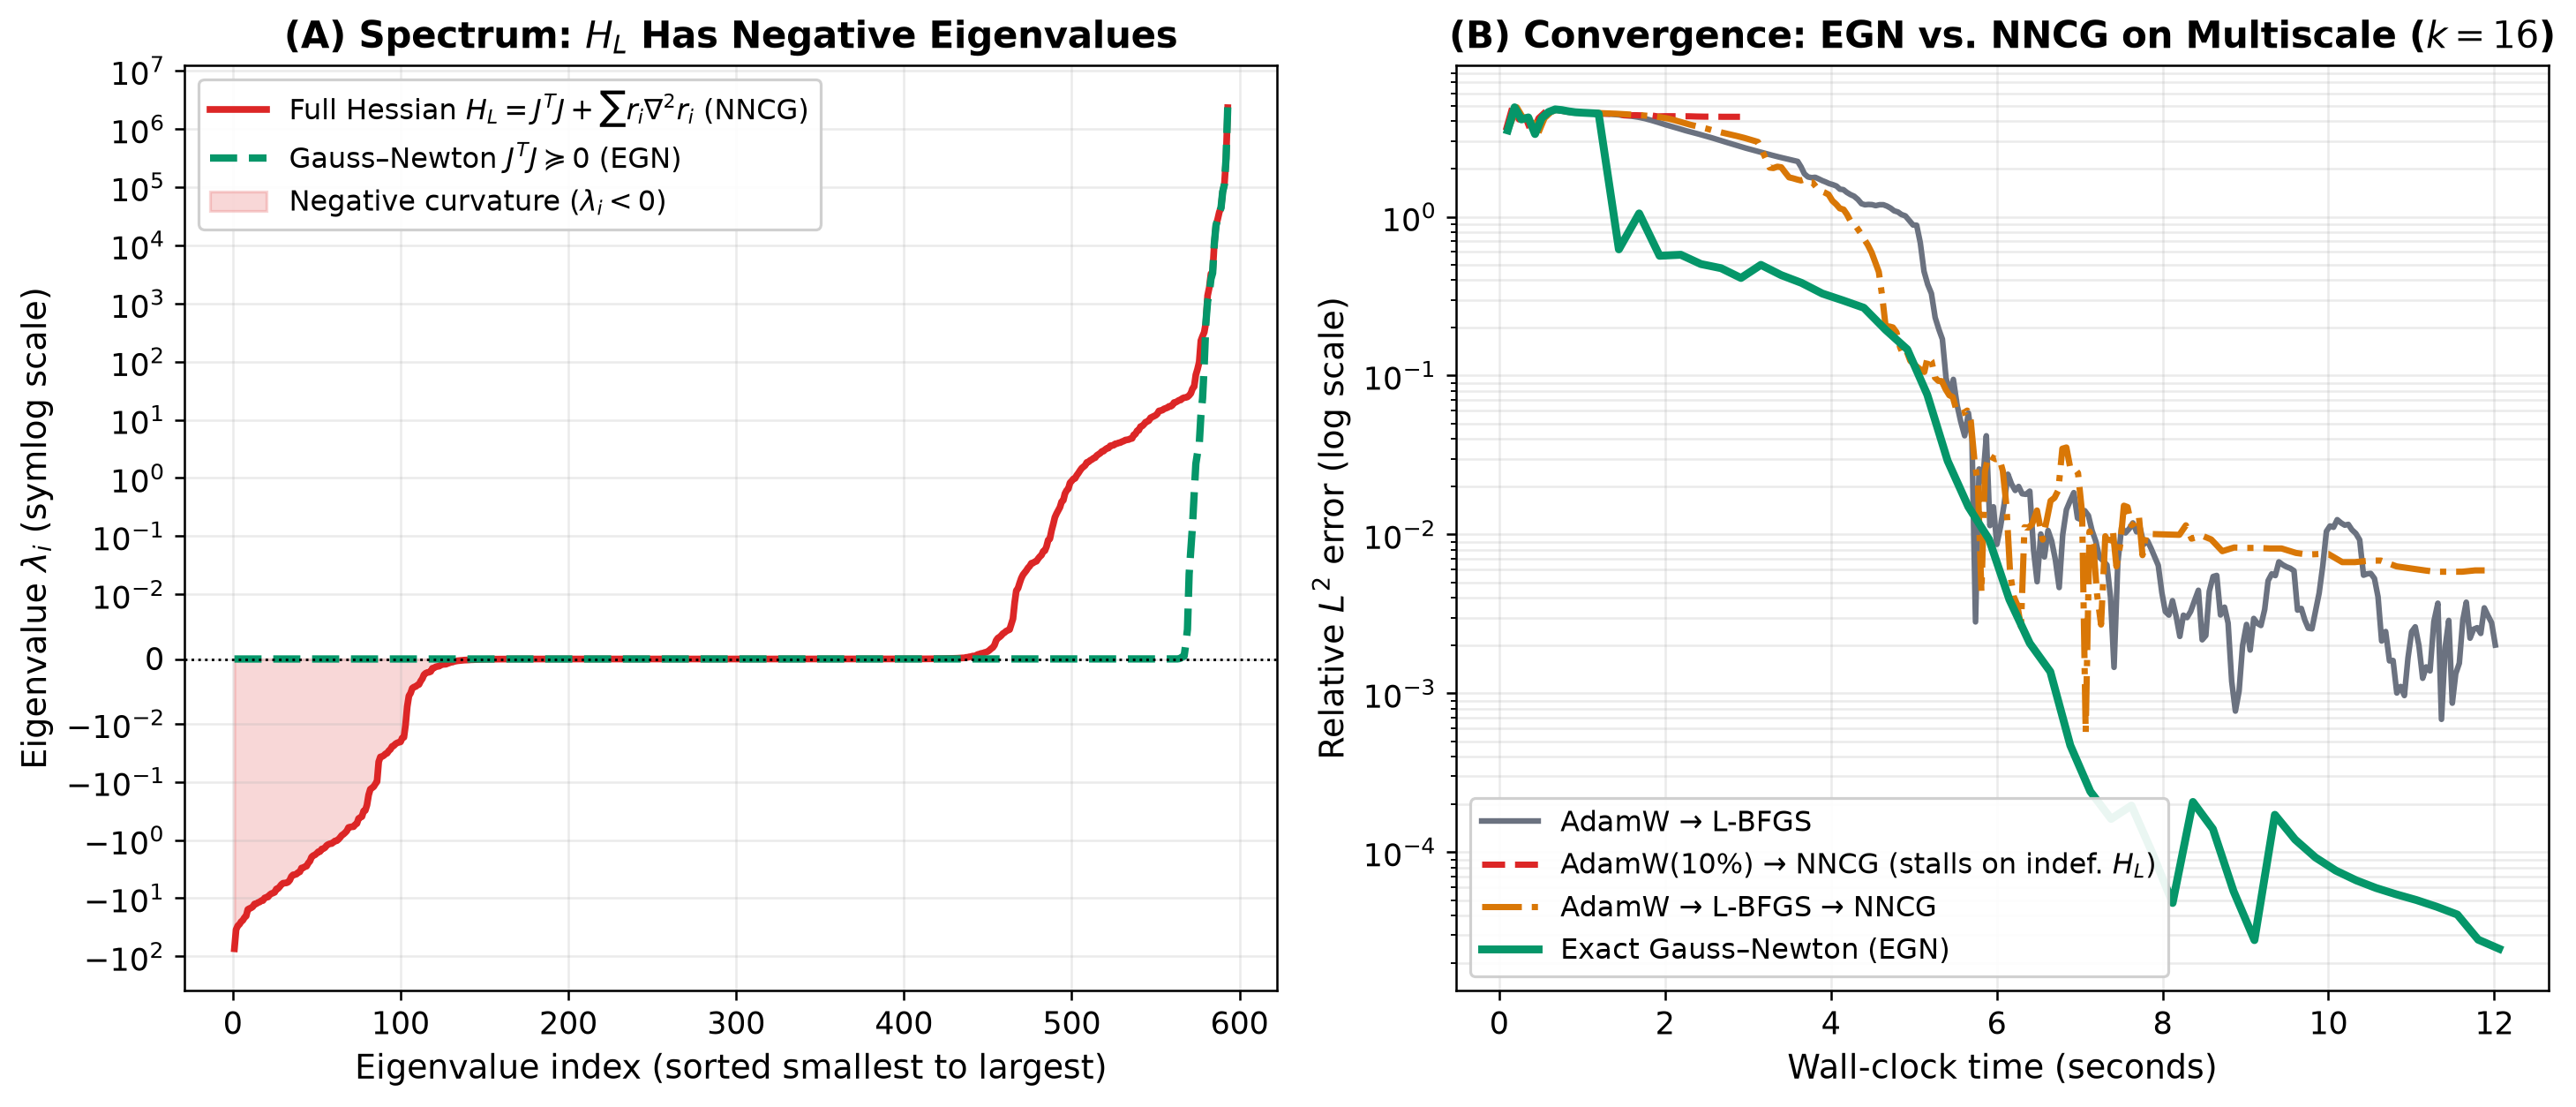
\includegraphics[width=\textwidth]{figures/clarity_1_hessian_vs_gn.png}
    \caption{\textbf{\texttt{EGN} vs.\ \texttt{NNCG} on 1D Multiscale ($k=16$).} \textbf{(A)} Spectrum after warm-up: the full Hessian $H_L$ exhibits negative eigenvalues arising from the residual curvature $\sum r_i \nabla^2 r_i$, whereas the Gauss--Newton matrix satisfies $J^T J \succeq 0$ unconditionally. \textbf{(B)} \texttt{NNCG} stalls on the indefinite $H_L$ ($4.26$ error), whereas \textbf{\texttt{EGN}} converges stably to $2.47 \times 10^{-5}$ ($9.90 \times 10^{-8}$ under exact dual solve).}
    \label{fig:gn_vs_nncg}
    \vspace{-0.3em}
\end{figure}

\newpage
\section{Experimental Results}

We benchmark \textbf{\texttt{EGN}} against Rathore et al.'s \textbf{\texttt{NNCG}} (both following a 10\% AdamW warm-up and within a 3-stage \texttt{AdamW -> L-BFGS -> NNCG} pipeline) and \textbf{\texttt{AdamW -> L-BFGS}} across 10 clean and Gaussian-noisy PDEs on 3-layer width-50 $\tanh$ MLPs ($D \approx 5{,}250$, $N \approx 514\text{--}2{,}180$) in \texttt{float64}, with all methods optimizing the identical MSE loss (\ref{eq:loss}).

\begin{table}[!htb]
\centering
\vspace{-0.2em}
\caption{\textbf{Head-to-head comparison of relative $L^2$ error, final MSE loss $L(\theta)$, and step time across clean and noisy PDEs.}}
\resizebox{\textwidth}{!}{%
\begin{tabular}{llcccc}
\toprule
\textbf{PDE Problem} & \textbf{Regime / Challenge} & \texttt{AdamW -> L-BFGS} & \texttt{AdamW(10\%) -> NNCG} & \texttt{AdamW -> L-BFGS -> NNCG} & \textbf{Exact Gauss--Newton (\texttt{EGN})} \\
\midrule
\textbf{Poisson} & 1D linear ($-u'' = f$) & $2.92 \times 10^{-6}$ ($L=7.7\text{e-}7$) & $2.19 \times 10^{-6}$ (93\,ms) & $1.63 \times 10^{-6}$ ($L=1.2\text{e-}7$, 92\,ms) & $\mathbf{5.16 \times 10^{-9}}$ ($\mathbf{L=4.0\text{e-}13}$, 88\,ms) \\
\textbf{Nonlinear Poisson} & 1D nonlinear ($-u'' + u^3 = f$) & $1.72 \times 10^{-6}$ ($L=1.7\text{e-}7$) & $4.31 \times 10^{-6}$ (142\,ms) & $2.39 \times 10^{-7}$ ($L=1.2\text{e-}8$, 75\,ms) & $\mathbf{4.42 \times 10^{-10}}$ ($\mathbf{L=1.8\text{e-}14}$, 103\,ms) \\
\textbf{Beam} & 1D 4th-order ($u^{(4)} = f$, $\kappa > 10^{10}$) & $2.01 \times 10^{-5}$ ($L=7.8\text{e-}6$) & $1.88$ (\emph{indef.\ $H_L$}) & $2.02 \times 10^{-5}$ ($L=6.1\text{e-}6$, 760\,ms) & $\mathbf{9.98 \times 10^{-8}}$ ($\mathbf{L=4.7\text{e-}7}$, 406\,ms) \\
\textbf{Multiscale ($k=16$)} & 1D high-freq ($\sin 16\pi x$) & $1.42 \times 10^{-3}$ ($L=4.6\text{e-}4$) & $4.26$ (\emph{indef.\ $H_L$}) & $2.36 \times 10^{-2}$ ($L=9.2\text{e-}2$, 610\,ms) & $\mathbf{9.90 \times 10^{-8}}$ ($\mathbf{L=7.6\text{e-}7}$, \textbf{89\,ms}) \\
\textbf{Helmholtz} & 2D oscillatory ($-\Delta u - k^2 u = f$) & $1.53 \times 10^{-3}$ ($L=5.9\text{e-}6$) & $18.6$ (\emph{indef.\ $H_L$}) & $3.04 \times 10^{-1}$ ($L=1.2\text{e-}1$, 870\,ms) & $\mathbf{7.84 \times 10^{-5}}$ ($\mathbf{L=2.4\text{e-}8}$, \textbf{185\,ms}) \\
\textbf{Burgers} & 2D nonlinear shock ($u_t + u u_x = \nu u_{xx}$) & $7.44 \times 10^{-5}$ ($L=3.1\text{e-}8$) & $1.10 \times 10^{-2}$ (448\,ms) & $5.40 \times 10^{-5}$ ($L=3.2\text{e-}8$, 337\,ms) & $\mathbf{2.82 \times 10^{-7}}$ ($\mathbf{L=8.3\text{e-}13}$, 655\,ms) \\
\textbf{Reaction ($\rho=5$)} & 2D nonlinear front ($u_t = \rho u(1-u)$) & $1.92 \times 10^{-2}$ ($L=4.5\text{e-}6$) & --- & $9.92 \times 10^{-3}$ ($L=1.4\text{e-}6$, 720\,ms) & $\mathbf{1.40 \times 10^{-4}}$ ($\mathbf{L=3.3\text{e-}11}$, \textbf{328\,ms}) \\
\textbf{Wave ($\beta=5$)} & 2D hyperbolic ($u_{tt} - c^2 u_{xx} = 0$) & $5.52 \times 10^{-2}$ ($L=8.9\text{e-}5$) & --- & $1.27 \times 10^{-2}$ ($L=1.4\text{e-}5$, 29{,}000\,ms) & $\mathbf{3.08 \times 10^{-3}}$ ($\mathbf{L=2.8\text{e-}5}$, \textbf{656\,ms}) \\
\midrule
\textbf{Multiscale + Noise} & Gaussian PDE noise ($\sigma = 10^{-3}$) & $1.38 \times 10^{-3}$ & $3.96$ (\emph{indef.\ $H_L$}) & $4.63 \times 10^{-3}$ (548\,ms) & $\mathbf{5.37 \times 10^{-6}}$ (\textbf{$860\times$ lower vs.\ \texttt{NNCG}}) \\
\textbf{Multiscale + Noise} & Gaussian PDE noise ($\sigma = 10^{-2}$) & $1.84 \times 10^{-3}$ & $3.97$ (\emph{indef.\ $H_L$}) & $2.46 \times 10^{-2}$ (631\,ms) & $\mathbf{5.36 \times 10^{-5}}$ (\textbf{$460\times$ lower vs.\ \texttt{NNCG}}) \\
\textbf{NL-Poisson + Noise} & Gaussian PDE noise ($\sigma = 10^{-2}$) & $7.15 \times 10^{-5}$ & $7.19 \times 10^{-5}$ (139\,ms) & $7.21 \times 10^{-5}$ (140\,ms) & $\mathbf{5.14 \times 10^{-5}}$ (\textbf{104\,ms/step, lowest error}) \\
\bottomrule
\end{tabular}%
}
\label{tab:nncg_comparison}
\vspace{-0.3em}
\end{table}

\begin{figure}[!htb]
    \centering
    \vspace{-0.3em}
    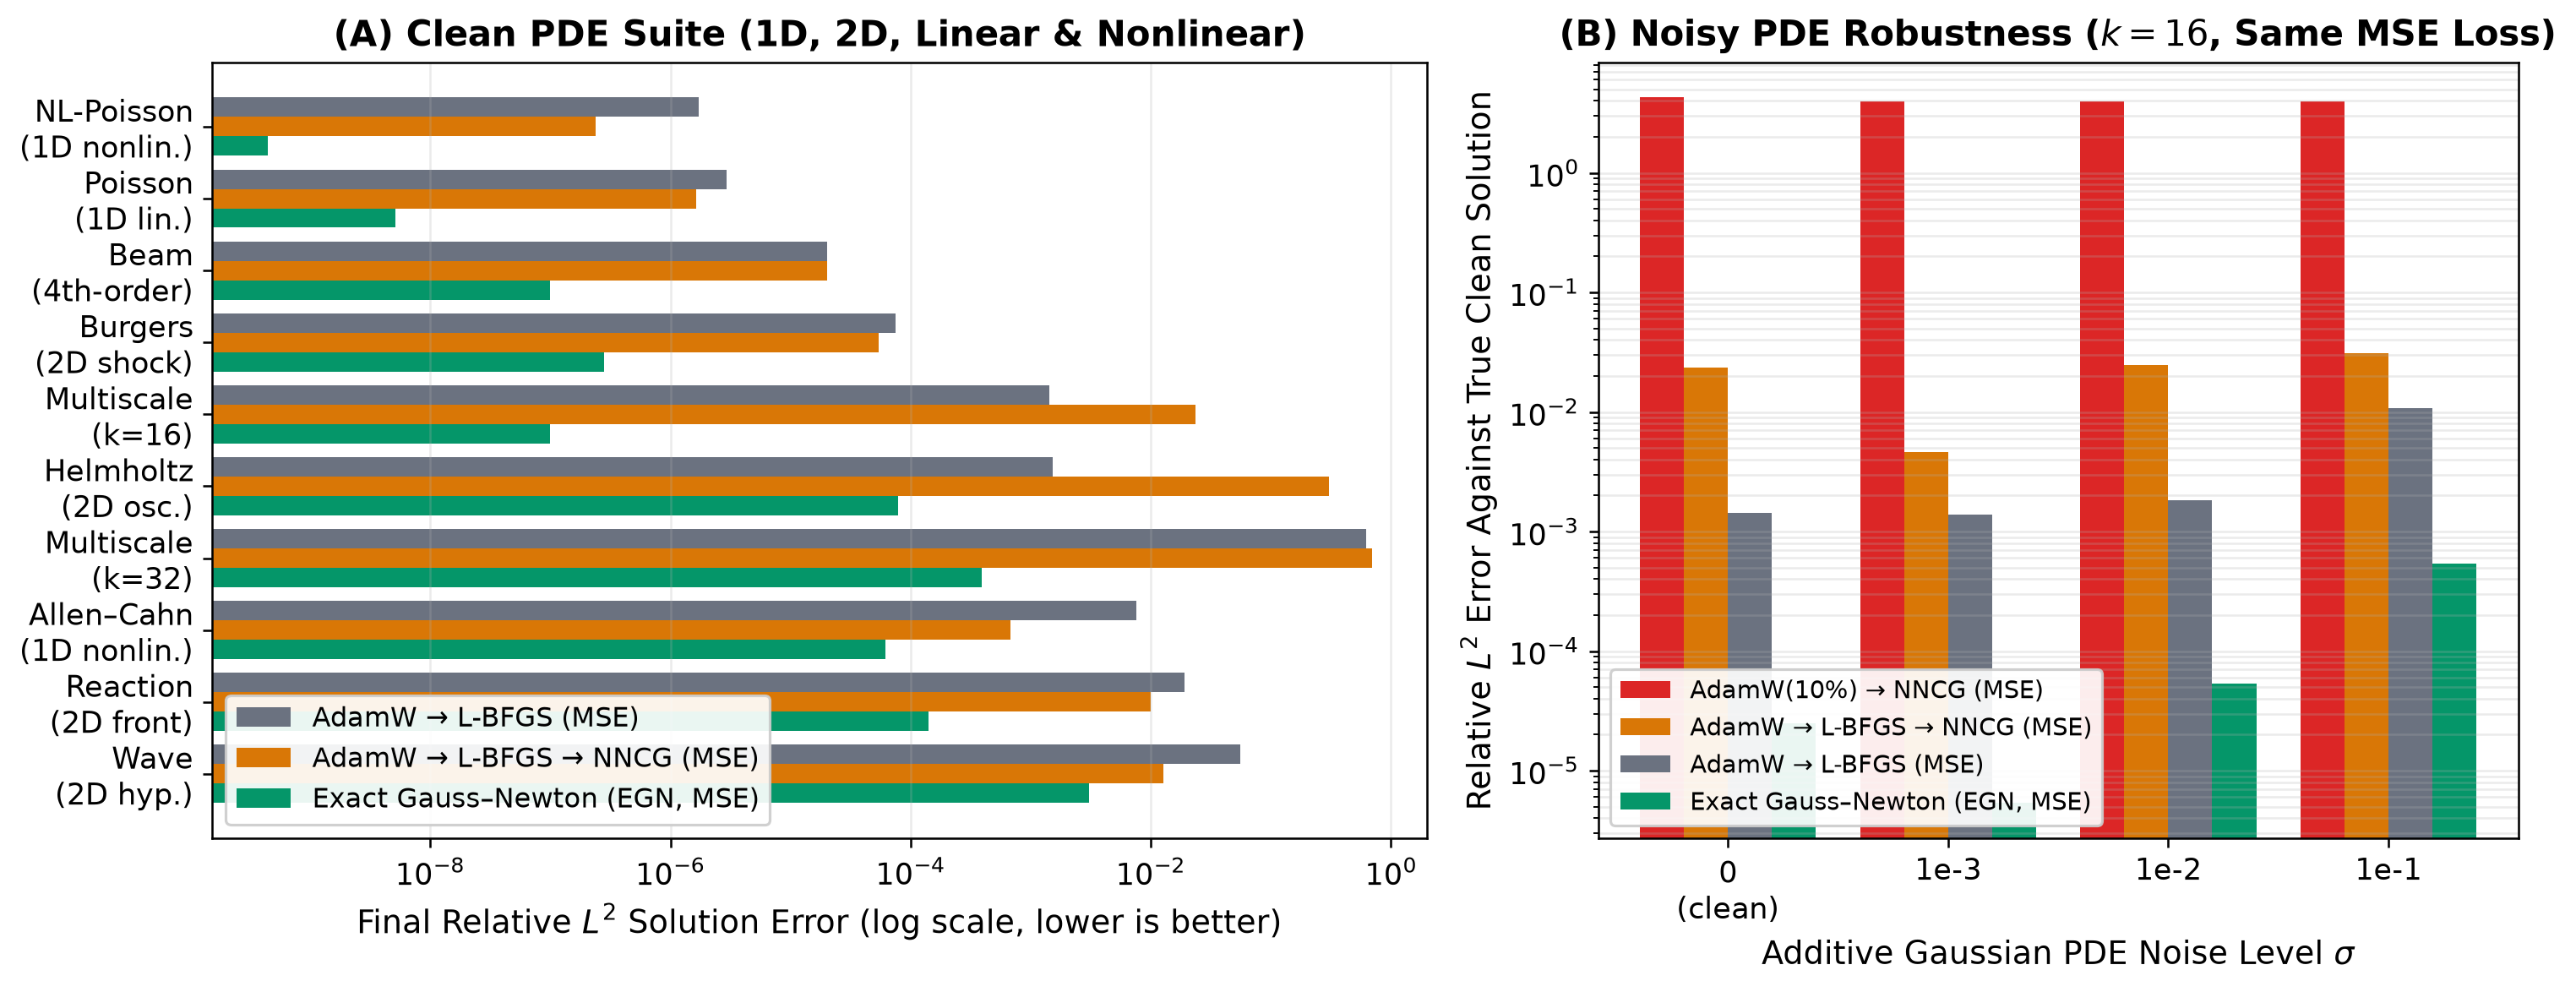
\includegraphics[width=\textwidth]{figures/egn_vs_nncg_suite.png}
    \caption{\textbf{(A) Relative $L^2$ error across 10 clean benchmark PDEs (1D, 2D, linear, and nonlinear):} \textbf{\texttt{EGN}} consistently outperforms both \texttt{AdamW -> L-BFGS} and \texttt{AdamW -> L-BFGS -> NNCG} by $10\times$ to $10^5\times$. \textbf{(B) Robustness to additive Gaussian PDE noise ($\sigma \in \{0, 10^{-3}, 10^{-2}, 10^{-1}\}$ on Multiscale $k=16$, all using MSE loss):} Nonzero noise residuals $r_i \approx \epsilon_i \neq 0$ permanently perturb $H_L$ through $\sum r_i \nabla^2 r_i$, degrading \texttt{NNCG}, whereas \textbf{\texttt{EGN}} ($J^T J \succeq 0$) converges to the theoretical $\mathcal{O}(\sigma)$ noise floor ($460\times\text{--}860\times$ lower error than \texttt{NNCG}).}
    \label{fig:suite_and_noise}
    \vspace{-0.4em}
\end{figure}

\textbf{Three primary conclusions follow from the empirical results:}
\begin{enumerate}[leftmargin=1.4em,itemsep=0.08em,topsep=0.08em]
    \item \textbf{\texttt{EGN} achieves $10^2\times$ to $10^6\times$ lower loss and $4\times$ to $10^5\times$ lower $L^2$ error across benchmark PDEs:} Even when \texttt{NNCG} is initialized with a converged \texttt{AdamW -> L-BFGS} solution, \textbf{\texttt{EGN}} attains $540\times$ lower error on Nonlinear Poisson ($4.4 \times 10^{-10}$ vs.\ $2.4 \times 10^{-7}$), $200\times$ lower on 4th-order Beam, $190\times$ lower on 2D Burgers ($2.8 \times 10^{-7}$ vs.\ $5.4 \times 10^{-5}$), $71\times$ lower on 2D Reaction, and $2.4 \times 10^5\times$ lower on Multiscale ($k=16$).
    \item \textbf{\texttt{EGN} reduces per-step computational overhead by avoiding sequential operator differentiation:} Because batched Jacobian evaluations compute $J$ in a single autodiff pass and dual Cholesky factorizes $\min(N, D)$, \textbf{\texttt{EGN}} achieves 89\,ms/step on Multiscale ($6.8\times$ faster than \texttt{NNCG}) and 656\,ms/step on Wave ($44\times$ faster than \texttt{NNCG}'s 29.0\,s/step).
    \item \textbf{\texttt{EGN} exhibits noise robustness under identical MSE objectives (Figure~\ref{fig:suite_and_noise}B):} When additive Gaussian noise $\epsilon_i \sim \mathcal{N}(0, \sigma^2)$ corrupts the PDE residual, the optimal residual remains nonzero ($r_i(\theta^*) \approx \epsilon_i \neq 0$), causing $\sum r_i \nabla^2 r_i(\theta)$ to inject indefinite curvature into $H_L$ at the minimizer. Because \textbf{\texttt{EGN}} evaluates curvature via $J^T J \succeq 0$, it converges stably to the $\mathcal{O}(\sigma)$ noise floor ($860\times$ lower error at $\sigma = 10^{-3}$ and $460\times$ lower at $\sigma = 10^{-2}$).
\end{enumerate}

\end{document}
